%!TEX root = ../template.tex
%%%%%%%%%%%%%%%%%%%%%%%%%%%%%%%%%%%%%%%%%%%%%%%%%%%%%%%%%%%%%%%%%%%%
%% chapter2.tex
%% UNIPD thesis document file
%%
%% Chapter with the template manual
%%%%%%%%%%%%%%%%%%%%%%%%%%%%%%%%%%%%%%%%%%%%%%%%%%%%%%%%%%%%%%%%%%%%

\typeout{NT FILE chapter2.tex}%

\chapter{SoundFood: {l'azienda e il contesto}}

\prependtographicspath{{Chapters/Figures/Covers/}}

Sebbene il panorama acustico raramente influenzi la scelta iniziale di un ristorante, può spesso determinare l'insoddisfazione dell'esperienza in esso. Il suono, infatti, non si limita a fungere da semplice sottofondo: è un elemento che influenza attivamente le nostre scelte.

Consideriamo dunque un nuovo concetto di ristorazione, dove la selezione musicale viene accuratamente studiata per creare una perfetta sintonia tra il gusto e l'ascolto.

È proprio da questa consapevolezza che nasce SoundFood, come risposta a un'esigenza specifica nel settore della ristorazione: migliorare l'esperienza del cliente attraverso l'integrazione di un elemento  spesso trascurato, il suono. Presentandosi come un "Phygital Music Sommelieer, l'azienda unisce le componenti fisiche e digitali per creare ambienti acustici su misura all'interno dei ristoranti. Il suo obiettivo va oltre la semplice fornitura di un dispositivo audio; cerca di trasformare il suono in un “condimento” coinvolgente che arricchisce e completa l'esperienza culinaria attraverso un sistema  dinamico che si adatta alle preferenze individuali del cliente e al contesto. \cite{soundfood2016}

Al centro di questa idea c’è il concetto di “bolle sonore”: microambienti acustici personalizzati per ogni tavolo, che consentono agli ospiti di immergersi in un'atmosfera musicale unica e priva di interferenze. Questi paesaggi sonori sono curati per arricchire i sapori di ogni piatto, supportati dall’integrazione di ricerche cross-modali che dimostrano come il suono possa influenzare la percezione del gusto e la soddisfazione generale.

La sinestesia sensoriale rappresenta il fondamento teorico di questa innovazione. Così come un film non può prescindere dalla sua colonna sonora, o un piatto dal suo corretto abbinamento enologico, anche l'esperienza gastronomica necessita di una propria dimensione sonora accuratamente studiata. L'impatto di questo approccio non è solo percettivo ma anche economico: i dati indicano che i ristoratori perdono circa il 23\% del potenziale fatturato al tavolo a causa di una inadeguata gestione sinestetica del suono, evidenziando come l'elemento acustico non sia solo una questione di comfort, ma un fattore determinante nella propensione alla spesa del cliente. \cite{negreira2019acoustics}

In un'epoca in cui l'esperienza gastronomica va oltre il semplice atto del mangiare, i ristoratori sono sempre più consapevoli della necessità di offrire un'esperienza completa per distinguersi in un mercato altamente competitivo.

Le realtà ristorative più esclusive al mondo dimostrano come la sinestesia non sia solo un elemento di contorno, ma una componente fondamentale dell'esperienza gastronomica contemporanea.

Il Sublimotion a Ibiza e l'Ultraviolet a Shanghai rappresentano esempi emblematici di questa evoluzione: più che ristoranti, si configurano come esperienze gastronomiche immersive dove ogni portata è accompagnata da un ambiente sensoriale completo, in cui suoni, proiezioni e illuminazioni si fondono con i sapori.

\begin{comment}
\begin{figure}[H]
    \centering
    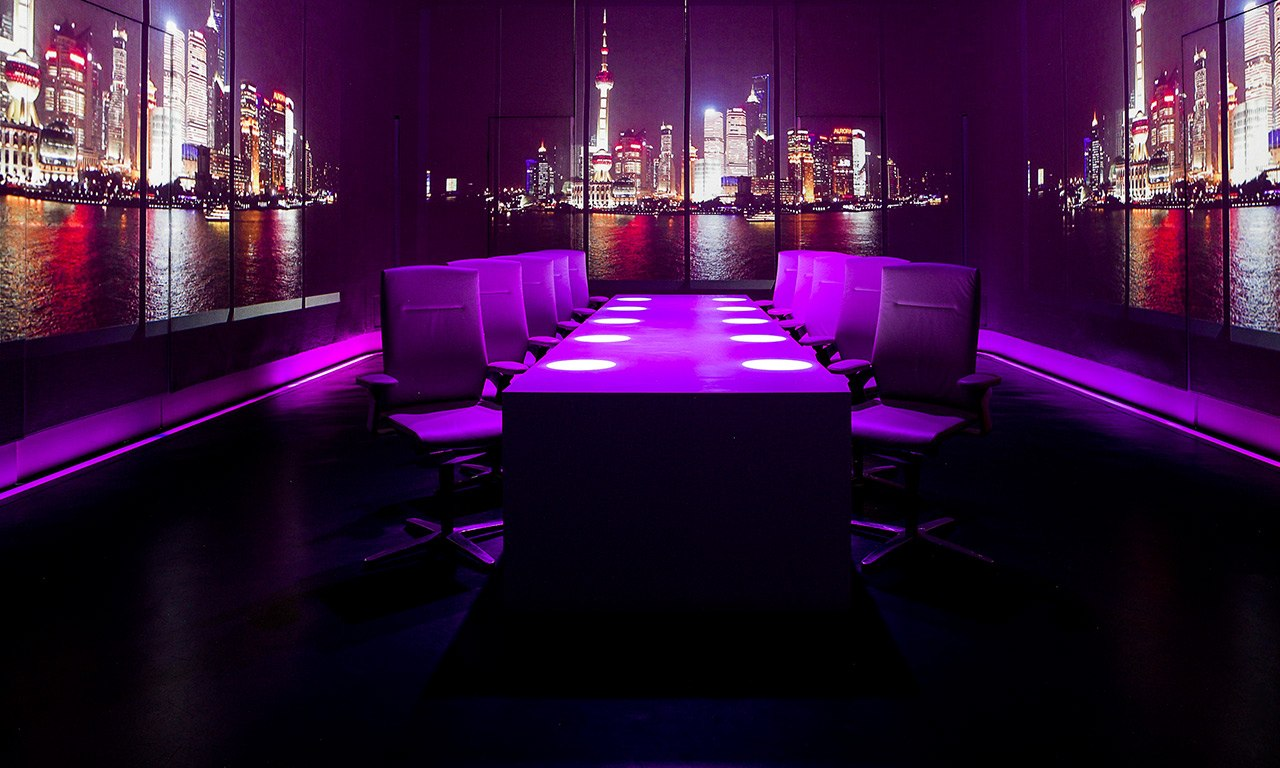
\includegraphics[width=0.5\textwidth]{Chapters/Figures/ultraviolet_shangai.jpg}
    \caption{\small Paul Pairet, Ultraviolet (2012), Shanghai}
    \label{fig:Ultraviolet}
\end{figure}
\end{comment}

Mentre queste realtà rappresentano l'apice dell'innovazione sensoriale nella ristorazione di lusso, SoundFood si propone di rendere accessibile questa tecnologia a una fascia più ampia di ristoranti, permettendo anche a realtà più tradizionali di arricchire l'esperienza dei propri clienti attraverso un approccio scientifico al sound design.

La tecnologia alla base di SoundFood supera i limiti delle soluzioni tradizionali, come l'utilizzo di auricolari o playlist generiche. Il sistema si basa su un'intelligenza artificiale che analizza e incrocia le caratteristiche organolettiche dei piatti con specifiche frequenze sonore, creando una proposta musicale personalizzata e scientificamente calibrata per ogni tavolo.

Questo sistema non solo migliora l'esperienza del cliente, ma offre anche al ristoratore uno strumento di gestione efficace e discreto, che non richiede interventi invasivi nella struttura del locale né modifica le abitudini di servizio del personale.